\chapter{The case of WASP-19b}\label{chap:wasp19}

\section{The system}
WASP-18b is a transiting hot Jupiter discovered by \citet{Hellier2009} within the WASP-South transit survey \citep{Pollacco2006}. It is an extremely close-in planet orbiting a F6 type star with a period of 0.94 days. Regarding its physical properties, WASP-18b is about ten times more massive than Jupiter with approximately the same size ($M_{P}=10.3\,{\rm M_{Jupiter}}$, $R_{P}=1.1\,{\rm R_{Jupiter}}$). Even though a rapid orbital decay was predicted theoretically \citep{Hellier2009}, it is not observed yet \citep{Wilkins2017} and new theoretical models proposed a variation of less than 4 seconds in the transit time over a 20-yr baseline
\citep{CollierCameron2018}.

\section{Transit Parameters and Physical Properties}
The results of the global fit of WASP-19 are listed in Table~\ref{tab:wasp19}, in comparison with the previous values from the discovery paper \citep{Hebb2010}, and a more recent work \citep{Lendl2013}. 

To estimate the stellar parameters of WASP-19, we used as priors the stellar spectroscopic parameters from \cite{Hebb2010}. Thus, in general, our results are in agreement with the those from the discovery paper. The most important discrepancies are the density of the star $\rho_*$ and the surface gravity $\log{g}$, showing $+2.5\sigma$ and $-3.2\sigma$ difference, respectively. Comparing with the results from \cite{Lendl2013}, ours are all in good agreement.

For values of the primary transit parameters obtained from the light curves, the greatest differences are found in the orbital inclination $i$ and the total transit duration $T_{14}$. We report an inclination value $5.1\sigma$ smaller than \cite{Hebb2010}, but in agreement with the estimate of \cite{Lendl2013}. In the other hand, our estimation of $T_{14}$ is significantly larger than \cite{Hebb2010} by $9\sigma$, but the difference is only $3.5\sigma$ when compared with \cite{Lendl2013}. We also report a preciser impact parameter $b$ and transit depth $\delta$.

As the same RV data set from the discovery paper \citep{Hebb2010} was used to perform our analysis, the almost identical values in the RV semi-amplitude $K$ is not a surprise. Moreover, the values from \cite{Lendl2013} are also in agreement. 

The planetary parameters derived from the light curve and radial velocity analysis are almost all in good agreement with the comparison works. The only parameter with a difference greater than $3\sigma$ is our estimation of the Equilibrium Temperature $T_{eq}$ compared with the result of \cite{Hebb2010}. However, our result is in better agreement with \cite{Lendl2013} by less than $2\sigma$.

\begin{landscape}
\begin{longtable}{llccc}
\caption{System parameter of WASP-19}
\label{tab:wasp19}
\centering
\tabularnewline
\hline 
~~~Parameter & Units & This work & \cite{Hebb2010}\footnote{a} & \cite{Lendl2013}\\
\hline
\smallskip\\\multicolumn{2}{l}{Stellar Parameters:}&\smallskip\\
~~~~$M_*$\dotfill &Mass (\(M_\odot\))\dotfill &$0.965^{+0.091}_{-0.095}$ & $0.95\pm0.10$ & $0.968^{+0.084}_{-0.079}$ \\
~~~~$R_*$\dotfill &Radius (\(R_\odot\))\dotfill &$1.006^{+0.031}_{-0.034}$ & $0.93^{+0.05}_{-0.04}$& $0.994\pm0.031$\\
~~~~$L_*$\dotfill &Luminosity (\(L_\odot\))\dotfill &$0.905^{+0.071}_{-0.069}$\\
~~~~$\rho_*$\dotfill &Density (cgs)\dotfill &$1.339^{+0.056}_{-0.058}$ & $1.19^{+0.12}_{-0.11}$\footnote{b}  & $1.384^{+0.055}_{-0.051}$\footnote{b}\\
~~~~$\log{g}$\dotfill &Surface gravity (cgs)\dotfill &$4.417^{+0.020}_{-0.021}$ & $4.48\pm0.03$\\
~~~~$T_{\rm eff}$\dotfill &Effective Temperature (K)\dotfill &$5616^{+66}_{-65}$ & $5500\pm100$\\
~~~~$[{\rm Fe/H}]$\dotfill &Metallicity \dotfill &$0.04^{+0.25}_{-0.30}$ & $0.02\pm0.09$\\
~~~~$Age$\dotfill &Age (Gyr)\dotfill &$6.4^{+4.1}_{-3.5}$ & $5.5^{+9.0}_{-4.5}$\\
%~~~~$d$\dotfill &Distance (pc)\dotfill &$270.2\pm1.7$\\

\smallskip\\\multicolumn{2}{l}{Planetary Parameters:}&\smallskip\\
~~~~$R_P$\dotfill &Radius (\rj)\dotfill &$1.415^{+0.044}_{-0.048}$ & $1.28\pm0.07$ & $1.376\pm0.046$\\
~~~~$M_P$\dotfill &Mass (\mj)\dotfill &$1.154^{+0.078}_{-0.080}$ & $1.14\pm0.07$ & $1.165\pm0.068$\\
~~~~$P$\dotfill &Period (days)\dotfill &$0.78883852^{+(75)}_{-(82)}$ & $0.7888399\pm(8)$  & $0.7888390\pm(2)$\\
~~~~$e$\dotfill &Eccentricity \dotfill &$0.0126^{+0.014}_{-0.0089}$ & & $0.0077^{+0.0068}_{-0.0032}$\\
~~~~$a$\dotfill &Semi-major axis (AU)\dotfill &$0.01652^{+0.00050}_{-0.00056}$ & $0.0164^{+0.0005}_{-0.0006}$ & $0.01653\pm0.00046$\\
~~~~$\omega_*$\dotfill &Argument of Periastron (Degrees)\dotfill &$51^{+89}_{-190}$ & $-76^{+112}_{-23}$ & $43^{+28}_{-67}$\\
~~~~$\rho_P$\dotfill &Density (cgs)\dotfill &$0.506^{+0.031}_{-0.030}$ & $0.54^{+0.07}_{-0.06}$& $0.595^{+0.036}_{-0.033}$\footnote{c}\\
~~~~$logg_P$\dotfill &Surface gravity \dotfill &$3.155^{+0.018}_{-0.019}$ & $3.20\pm0.03$ & $3.184\pm0.015$\\
~~~~$T_{eq}$\dotfill &Equilibrium temperature (K)\dotfill &$2113\pm29$ & $1993^{+32}_{-33}$ & $2058\pm40$\\
~~~~$\Theta$\dotfill &Safronov Number \dotfill &$0.0279^{+0.0012}_{-0.0011}$\\
~~~~$\fave$\dotfill &Incident Flux (\fluxcgs)\dotfill &$4.52^{+0.26}_{-0.24}$\\

\smallskip\\\multicolumn{2}{l}{Primary Transit Parameters:}&\smallskip\\
~~~~$T_0$\dotfill & Transit Time (\bjdtdb)\dotfill &$2456402.7128^{+(17)}_{-(14)}$ & $2454775.3372\pm(2)$ & $2456029.59204\pm(13)$\\
~~~~$i$\dotfill &Inclination (Degrees)\dotfill &$79.08^{+0.34}_{-0.37}$ & $80.8\pm0.8$  & $79.54\pm0.33$\\
~~~~$R_P/R_*$\dotfill &Radius of planet in stellar radii \dotfill &$0.14410^{+0.00049}_{-0.00050}$ & $0.1425\pm0.0014$\\
~~~~$a/R_*$\dotfill &Semi-major axis in stellar radii \dotfill &$3.533^{+0.048}_{-0.052}$ &  & $3.573\pm0.046$\\
~~~~$b$\dotfill &Impact parameter \dotfill &$0.6671^{+0.0087}_{-0.0091}$ & $0.62\pm0.03$ & $0.645\pm0.012$\\
~~~~$\delta$\dotfill &Transit depth (fraction)\dotfill &$0.02077\pm0.00014$ & $0.0203\pm0.0004$ & $0.02018\pm0.00021$\\
~~~~$u_{1,I}$\dotfill &linear LD coeff., I band\dotfill &$0.287^{+0.027}_{-0.029}$&\\
~~~~$u_{2,I}$\dotfill &quadratic LD coeff., I band\dotfill &$0.263\pm0.024$&\\
~~~~$u_{1,R}$\dotfill &linear LD coeff., R band \dotfill &$0.383^{+0.029}_{-0.032}$\\
~~~~$u_{2,R}$\dotfill &quadratic LD coeff., R band\dotfill &$0.246^{+0.027}_{-0.025}$\\
~~~~$T_{14}$\dotfill &Total transit duration (days)\dotfill &$0.06697^{+0.00031}_{-0.00030}$ & $0.0643^{+0.0006}_{-0.0007}$ & $0.06586^{+0.00033}_{-0.00031}$\\
~~~~$P_T$\dotfill &A priori non-grazing transit prob \dotfill &$0.2426^{+0.0066}_{-0.0051}$\\
~~~~$P_{T,G}$\dotfill &A priori transit prob \dotfill &$0.3246^{+0.0089}_{-0.0069}$\\
~~~~$\tau$\dotfill &Ingress/egress transit duration (days)\dotfill &$0.01459\pm0.00035$\\

\smallskip\\\multicolumn{2}{l}{RV Parameters:}&\smallskip\\
~~~~$e\cos{\omega_*}$\dotfill & \dotfill &$-0.0027^{+0.0077}_{-0.013}$ & $0.004\pm0.009$ &$0.0024\pm0.0020$ \\
~~~~$e\sin{\omega_*}$\dotfill & \dotfill &$0.0016^{+0.014}_{-0.0092}$ & $-0.02\pm0.02$ & $0.000\pm0.005$\\
~~~~$K$\dotfill &RV semi-amplitude (m/s)\dotfill &$255.4^{+6.1}_{-6.2}$ & $256\pm5$  & $257.7\pm2.9$\\
~~~~$M_P\sin i$\dotfill &Minimum mass (\mj)\dotfill &$1.133^{+0.078}_{-0.079}$\\

\smallskip\\\multicolumn{2}{l}{Secondary Eclipse Parameters:}&\smallskip\\
~~~~$T_S$\dotfill &Time of eclipse (\bjdtdb)\dotfill &$2455169.3621^{+(41)}_{-(51)}$ & $2456030.77766\pm(88)$\\
~~~~$b_S$\dotfill &Eclipse impact parameter \dotfill &$0.670^{+0.020}_{-0.017}$ & $0.652\pm0.015$\\
~~~~$\tau_S$\dotfill &Ingress/egress eclipse duration (days)\dotfill &$0.01472^{+0.00085}_{-0.00066}$\\
~~~~$T_{S,14}$\dotfill &Total eclipse duration (days)\dotfill &$0.06812^{+0.00087}_{-0.00074}$\\
~~~~$P_S$\dotfill &A priori non-grazing eclipse prob \dotfill &$0.2415\pm0.0021$\\
~~~~$P_{S,G}$\dotfill &A priori eclipse prob \dotfill &$0.3232\pm0.0030$\\
\hline
%\end{tabular}
%\tablefoot{
%\tablefoottext{a}{For comparison, the results from \cite{Hellier2009} that considered free eccentricity were used.}
%%\tablefoottext{b}{Values converted to cgs units multiplying by the Sun density $\rho_{\odot}=1.408\,$cgs.}
%\tablefoottext{c}{Values converted to cgs units multiplying by the Jupiter density $\rho_{J}=1.33\,$cgs}
%\tablefoottext{d}{Values enclosed in parentheses correspond to the uncertainties of the last digits of the nominal value.}}
\end{longtable}
\end{landscape}

\section{Transit Timing Variations}

The proposed equation for linear ephemeris, considering 59 transit times of WASP-19b is:
\begin{equation} \label{eq1_w19}
T_{\rm C}(E)=2456402.7128\pm(16)+E \cdot 0.788838858\pm(47)
\end{equation}

The TTV values from the proposed linear ephemeris are listed in Table \ref{times_wasp19}, including transit times from the previous works \citep{Hebb2010,Anderson2010,Lendl2013,Tregloan2013,Bean2013,Mancini2013}. 

At the middle panel of Figure XXX are the TTV values versus epoch, for all the transit time considered in this work.

The RMS from the linear ephemeris is about 75 seconds. The epoch of $-1011$ is the only one with a transit time deviation above $1.5\,\sigma$ from the linear ephemeris. If it is removed, then the RMS decreases to 69 seconds. Moreover, in our data the epoch $-611$ has one of the greatest errors due to bad weather conditions.

Considering all the transit times from Table~\ref{times_wasp19}, the linear fit has $\chi^{2}_{red} = 0.16$. This an indication of an overestimation of the errors. A second degree polynomial was also tested in order to reject or not a possible orbital decay. The goodness of that fit is $\chi^{2}_{red}=0.12$. 

%\begin{longtable}[H]

\begin{longtable}{cccc}
\caption{Transit mid-times for WASP-19b}
\label{times_wasp19}
\tabularnewline
\hline \hline
Epoch & Transit mid-time & TTV & References\\
      & (${\rm BJD_{TDB}}$) & (min) &  \\
\hline
-2063 & $2454775.3372$ & $-1.6\pm3.2$ & 1\\
-2061 & $2454776.91566$ & $-0.5\pm2.3$ & 2 \\
-2010 & $2454817.14633$ & $-0.6\pm2.3$ & 3 \\
-1525 & $2455199.73343$ & $-0.2\pm2.6$& 4\\
-1459 & $2455251.79657$ & $-0.6\pm2.3$& 5 \\
-1458 & $2455252.58544$ & $-0.5\pm2.3$& 5 \\
-1454 & $2455255.74077$ & $-0.6\pm2.3$& 5 \\
-1449 & $2455259.68448$ & $-1.3\pm2.4$& 4 \\ 
-1431 & $2455273.88282$ & $-2.4\pm2.5$& 4 \\
-1399 & $2455299.12768$ & $0.6\pm2.4$& 4 \\
-1354 & $2455334.6254$ & $0.5\pm2.3$ & 6\\
-1349 & $2455338.56927$ & $0.1\pm2.3$& 3 \\ 
-1330 & $2455353.55659$ & $-0.8\pm2.3$& 6\\
-1317 & $2455363.81131$ & $-1.1\pm2.4$& 4  \\
-1311 & $2455368.54285$ & $-3.3\pm3.8$& 6 \\ 
-1094 & $2455539.72327$ & $0.2\pm2.4$ & 3 \\
-1056 & $2455569.69826$ & $-1.1\pm2.4$ & 3\\
-1039 & $2455583.10979$ & $0.8\pm2.6$ & 4 \\
-1037 & $2455584.68693$ & $0.0\pm2.3$ & 3 \\
-1025 & $2455594.15188$ &  $-1.6\pm3.3$ & 6 \\
-1016 & $2455601.25164$ & $-1.3\pm2.5$ & 6\\
-1014 & $2455602.83138$ & $1.7\pm2.4$ & 3 \\
-1011 & $2455605.19414$ & $-3.8\pm3.5$ & 6 \\
-1009 & $2455606.77464$ & $0.3\pm2.3$ & 3 \\
-1008 & $2455607.56241$ & $-1.2\pm2.4$ & 3 \\
-989 & $2455622.55057$ & $-0.9\pm2.3$ & 3 \\
-987 & $2455624.12787$ & $-1.5\pm3.1$ & 6 \\
-976 & $2455632.80612$ & $0.0\pm2.3$ & 3 \\
-947 & $2455655.68222$ & $-0.3\pm2.4$ & 3 \\
-928 & $2455670.66976$ & $-0.9\pm2.5$ & 3 \\
-923 & $2455674.61367$ & $-1.3\pm2.4$ & This work \\
-919 & $2455677.77038$ & $0.7\pm3.6$ & 6  \\
-905 & $2455688.81201$ & $-2.4\pm5.3$ & 6 \\
-904 & $2455689.60276$ & $0.4\pm2.4$ & 6 \\
-900 & $2455692.75674$ & $-1.6\pm4.3$ & 6 \\
-899 & $2455693.54639$ & $-0.5\pm2.3$ & 6  \\
-886 & $2455703.79933$ & $-3.3\pm6.4$ & 6 \\
-885 & $2455704.59078$ & $0.5\pm2.4$ & 6 \\
-880 & $2455708.534626$ & $0.0\pm 2.3$ & 6  \\
-654 & $2455886.81234$ &  $0.2\pm3.8$ & 6 \\
-642 & $2455896.27611$ & $-3.1\pm3.8$ & 6 \\
-618 & $2455915.20980$ & $-0.9\pm2.5$ & 6  \\
-613 & $2455919.15485$ & $0.4\pm 2.7$ & 6\\
-611 & $2455920.7353$ & $0.0\pm5.4$ & This work \\
-609 & $2455922.30966$ & $-0.4\pm8.3$ & 6 \\
-511 & $2455999.6163$ & $0.2\pm2.3$ & 7 \\
-483 & $2456021.70374$ & $0.1\pm2.3$ & 7 \\
-473 & $2456029.5925$ & $0.7\pm 2.4$ &3 \\
-468 & $2456033.53643$ &  $0.3\pm 2.3$ & 6  \\
-430 & $2456063.51174$ & $-0.5\pm 2.3$ & 3 \\
-86 & $2456334.87208$ & $-0.8\pm2.4$ & 4 \\
-47 & $2456365.6373$  & $-0.1\pm2.3$& This work \\
1 & $2456403.50158$ &  $-0.1\pm2.3$ & This work \\
729 & $2456977.77722$  & $1.3\pm2.3$ & 8 \\
867 & $2457086.63571$ & $-0.5\pm2.3$& This work \\
1383 & $2457493.67676$   & $-0.2\pm2.3$& This work  \\
1771 & $2457799.74612$ &  $-0.3\pm2.3$ & This work \\
1838 & $2457852.597807$ & $-0.7\pm2.3$ & This work\\ 
2064 & $2458030.8751$  & $-1.5\pm3.2$& This work \\
\hline
%\end{tabular}
%\tablebib{(1)~\citet{Hebb2010};
%(2) \citet{Anderson2010}; (3) \citet{Lendl2013}; (4) Exoplanet Transit Database (ETD) \url{var2.astro.cz/ETD}; (5) \citet{Tregloan2013}; (6) \citet{Mancini2013}; (7) \citet{Bean2013}; (8) \citet{Sedaghati2015}.}
\end{longtable} 

\section{Limits on an additional perturber}

For the WASP-19b system the measured transit-timing RMS scatter was $\rm TTV_{\rm RMS}=75,\rm s$. Additional bodies with a mass of $500~M_{\oplus}$ and as low as $2.0~M_{\oplus}$ and $0.9~M_{\oplus}$ at the 1:3, 1:2 (interior) and 2:1 (exterior) mean-motion resonances could cause the observed RMS scatter. Hypothetical planets of $6~M_{\oplus}$, $3~M_{\oplus}$ and $2~M_{\oplus}$ could cause the observed RMS scatter at the 5:3, 5:2 and 3:1 exterior mean-motion resonances, respectively. We refer to Fig.~\ref{megno_wasp19}.

\begin{figure}
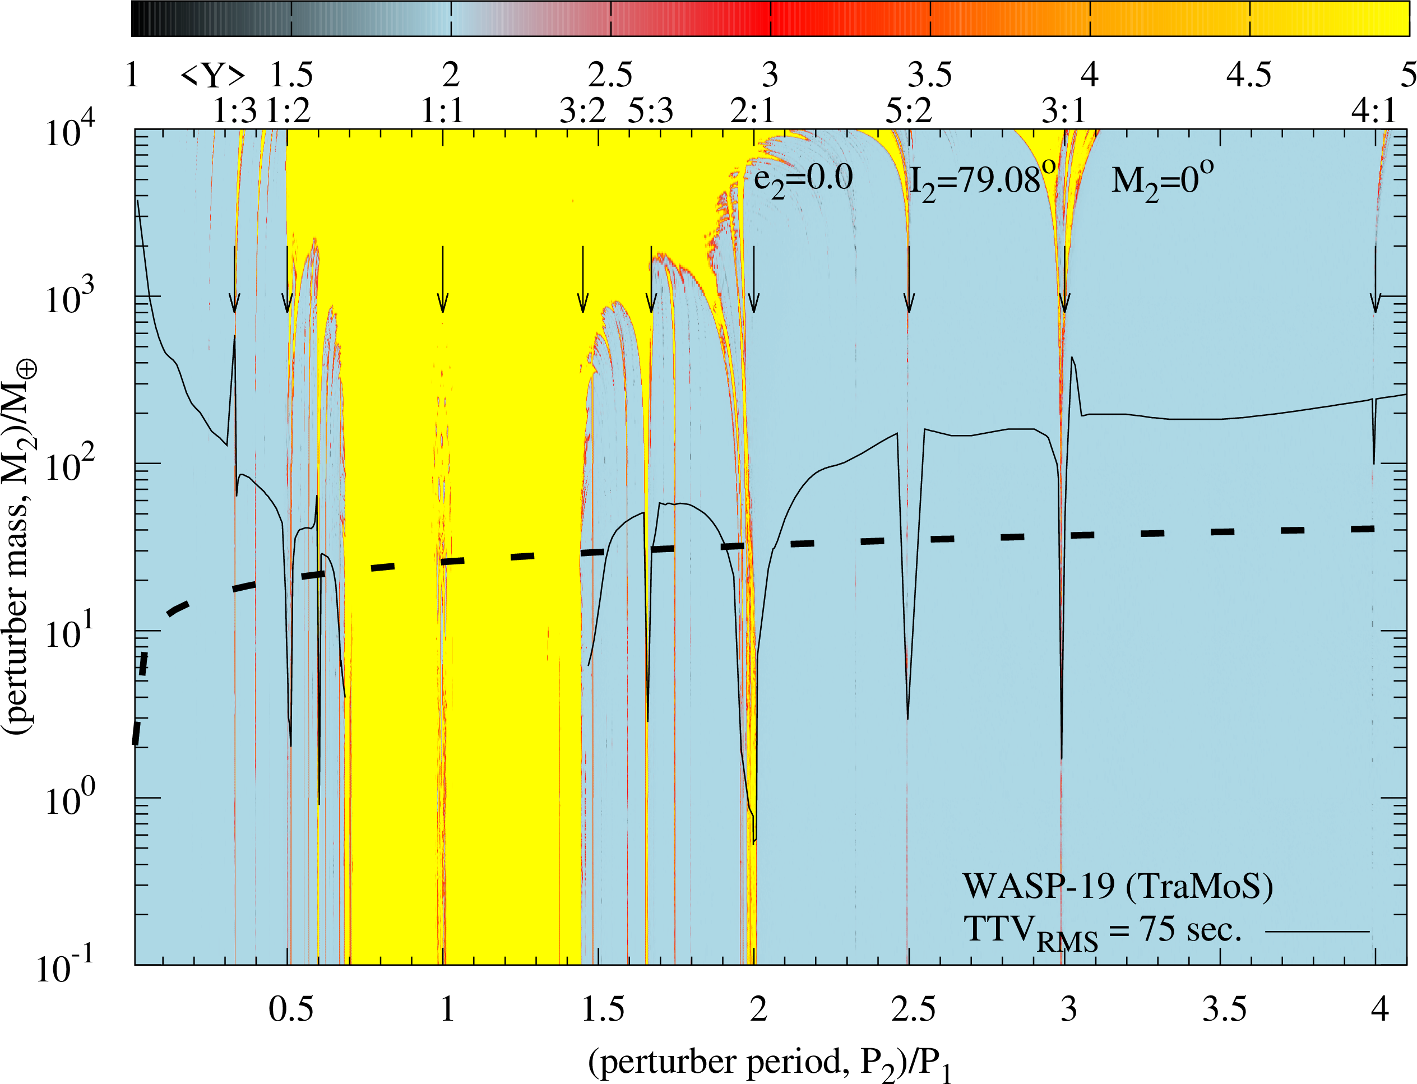
\includegraphics[width=1.0\columnwidth]{imagenes/WASP19_TraMos_Map001_GIMP_scaled.png}
\caption{Same as Fig.~\ref{megno_wasp18}, but this time for WASP-19 with an $\rm TTV_{\rm RMS}$ of 75 s. The
RMS for the radial-velocity measurements was $(18.2\,\rm m/s)$. \emph{See electronic version for colors}.}
\label{megno_wasp19}
\end{figure}